\chapter{Working with Sprites}
Sprites are likely the most important component of any 2D game. A Sprite is
simply the representation of a game object on the screen. If you add a Sprite to
a Scene in \cocos{} it will be rendered and the texture of the Sprite will be
visible within the game. 

Almost all \cocos{} classes use a \inlinecode{CC} prefix. The class that is used
to create Sprites in \cocos{} is called \inlinecode{CCSprite}. Whenever you want
to draw an object to the screen you will use a \inlinecode{CCSprite}.

In this chapter you start working on your first game! Throughout setting the
game you will learn all the basics about Sprites in \cocos{}. Let's get started!

\section{Setting up your first \cocos{} project}
We are going to create this game entirely in \xcode{} not using SpriteBuilder. You
will learn how to use SpriteBuilder throughout the next example games. 
Setting a \cocos{} project up is easy - open \xcode{} and select \textit{File >
New Project}:

\begin{figure}[H]
		\centering
		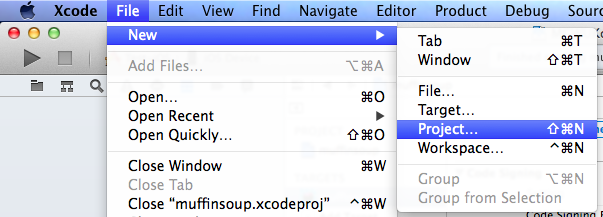
\includegraphics[width=280pt]{images/sprites/xcode_new_project.png}     
		\caption{Your first \cocos{} project!}
\end{figure}

Now you need to choose a project template. You need to select the \cocos{}
template. The \cocos{} template will set you up with a project that already has
\cocos{} and and two scenes included.

\begin{figure}[H]
		\centering
		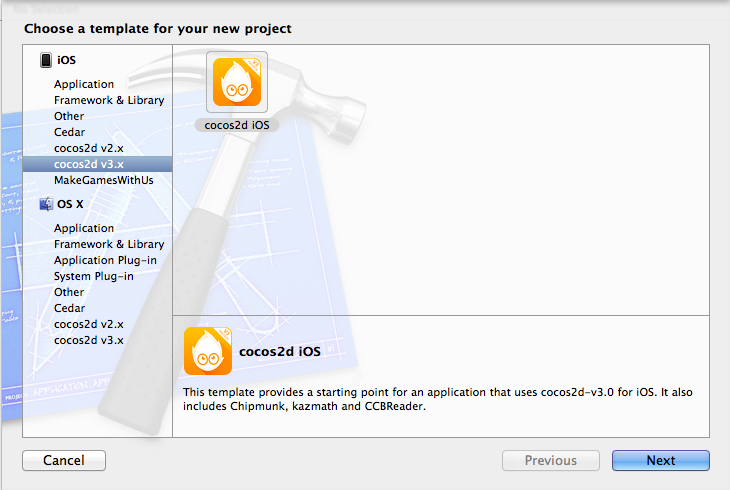
\includegraphics[width=280pt]{images/sprites/new_cocos_project.png}     
		\caption{Your first \cocos{} project!}
\end{figure}

We're not completely through the setup process yet. In the next step you need to
choose a name for your project. It is going to be \textit{Falling Apples}:

\begin{figure}[H]
		\centering
		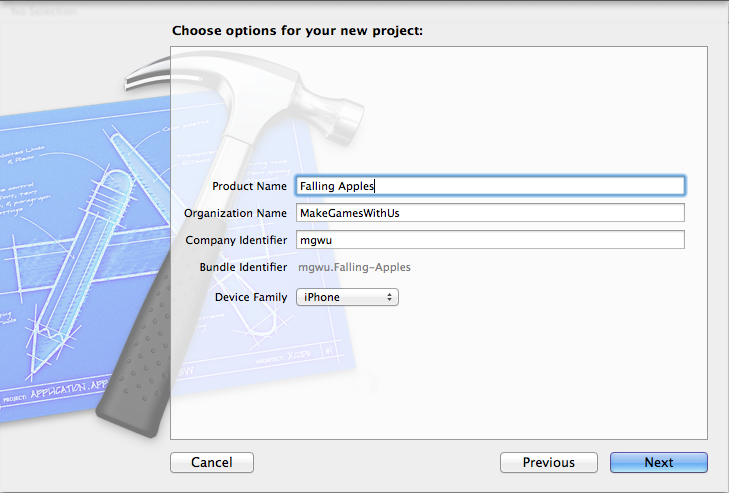
\includegraphics[width=280pt]{images/sprites/xcode_fallingapples.png}     
		\caption{Your first \cocos{} project!}
\end{figure}

Now there's one last step and we're finally ready to code! Choose a location on
your hard drive to store the project. I always recommend having a
\textit{Development} folder to keep all your coding projects in one place.
Choose whichever location you like and select the \textit{Create} button.

Now you will see the \cocos{} template project in \xcode{}. Let's run the
project to see that everything works. In the top left corner you will see an
area that is dedicated to run apps on different devices or simulators. You need
to run the \textit{FallingApples} project on the \textit{iPhone Retina (4-inch)
> iOS 7} Simulator. If a different iPhone simulator is selected you can change
that by clicking onto the displayed name of the current iPhone simulator.

\begin{figure}[H]
		\centering
		
\includegraphics[width=280pt]{images/sprites/run.png}     
		\caption{Your first \cocos{} project!}
\end{figure}


You now should be ready to run the game! Once you hit the run button you get to
see this:

\begin{figure}[H]
		\centering
		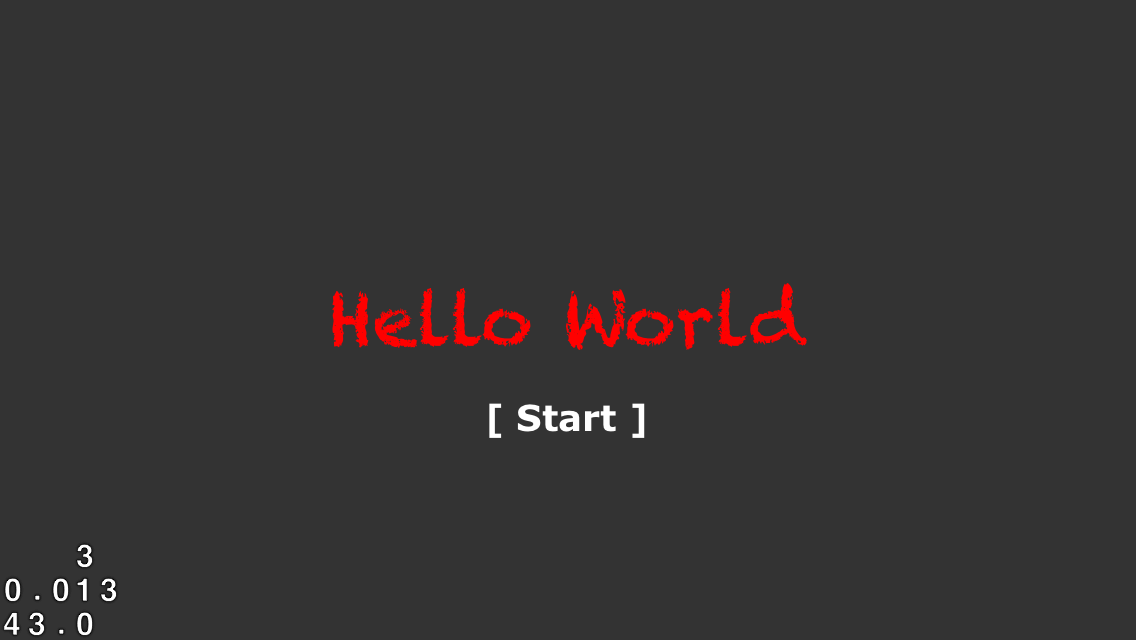
\includegraphics[width=280pt]{images/sprites/template_screenshot.png}     
		\caption{The first scene in our game}
\end{figure}

This is the first scene of your game (We will get into the concept of scenes
later on)! The content you can see on the screen has been created by the
\cocos{} template.

The code for this first scene is within the class called
\inlinecode{IntroScene}. Open \textbf{IntroScene.m} to take a look at it.

We want to start with a blank project and learn everything from scratch. So the
first thing we will do is remove most of the content from \textbf{IntroScene.m}.
 
\begin{lstlisting}[title=IntroScene.m]
#import "IntroScene.h"
#import "HelloWorldScene.h" 

@implementation IntroScene

+ (IntroScene *)scene
{
  return [[self alloc] init];
}

- (id)init
{
  self = [super init];  
  if (self) {
    // we will place our setup code here
  }
  return self;
}
@end
\end{lstlisting}

Once you applied the changes and removed most of the code in
\inlinecode{IntroScene} we are ready to start working on our falling objects
game!

\begin{lamp}[frametitle={About Code Snippets}]
Most Code Snippets in this book will only contain code and other relevant parts
of a file. In many cases we will omit some of the comments in the source file to
make the code more readable in a book format.
\end{lamp}

\section{Adding Resources to your game}
This chapter is all about Sprites and displaying images within a game. The first step we need to tackle is actually adding
some images to our game that we can use to texture Sprites. We have prepared some
assets for this game, you can download them from \ldots. \todo{Add actual links to the resources that should be downloaded}

Once you have downloaded the images you need to add them to your Xcode project.
\todo{Explain with screenshots once we have images}

Well done! Now we can use the images within our game.

\section{Creating a Sprite}
Now it's time to actually create a Sprite and render it on the screen. 
The easiest way to setup a textured Sprite is the following line of
code. Add it to the \inlinecode{init} method within the \inlinecode{if
(self){\ldots}} block:

\begin{lstlisting}
CCSprite *fallingObject = [CCSprite spriteWithImageNamed:@"apple.png"];
\end{lstlisting}

The code for this is really simple, using the \inlinecode{spriteWithImageNamed}
method \cocos{} will automatically search for the image in all subfolders you
have included in your project and initialize a \inlinecode{CCSprite} with that
texture.
\begin{error}
It is very convenient that you don't have to provide a path to the images you
want to use. But be careful, you should never add multiple images with the same
name otherwise there will be no way for \cocos{} to decide which image you are
referring to.\todo{Verify if path can be provided optionally to differentiate
two images with the same name}.
\end{error}

Now we have created a Sprite but we still need to let \cocos{} know that it
shall be rendered. By default \cocos{} renders everything that is part of the
current scene graph - that means it will render all children (and children of
children, etc.) of the current scene. Scenes will be discussed in detail
throughout this book, for now it is important to know that:
\begin{itemize}
  \item Scenes are represented by the class \inlinecode{CCScene}
  \item Scenes always have the size of the full screen
  \item The only scene we are using in the current project is
  \inlinecode{IntroScene}
  \item Scenes can have children. All children of an active scene will be
  displayed on the screen.
\end{itemize}

Now that we have created a sprite we need to add it to the
\inlinecode{IntroScene} so that we can see it on the screen. 
\begin{lstlisting}
[self addChild:fallingObject];
\end{lstlisting}
Add the above line to the \inlinecode{init} method, after the line that creates
the falling object.

Now your \inlinecode{init} method should look like this:
\begin{lstlisting}
- (id)init
{
  self = [super init];
    
  if (self) {
    CCSprite *fallingObject = [CCSprite spriteWithImageNamed:@"apple.jpeg"];
    [self addChild:fallingObject];
  }
  
  return self;
}
\end{lstlisting} 
\inlinecode
\subsection{Different devices - different resources}

\texttt{spriteWithImageNamed:} utilizes \texttt{CCFileUtils} to
automatically find the image in the right resolution, you do not have to
specify the resolution manually. The line above also works for images
contained in \emph{Smart Sprite Sheets} created by SpriteBuilder. In
case you are using folders in SpriteBuilder you need to include the
complete path to the image, e.g.:

\begin{verbatim}
CCSprite *hero = [CCSprite spriteWithImageNamed:@"gameAssets/hero.png"];
\end{verbatim}

The content size of the sprite will automatically be the size of the
texture.

\subsection{Changing the texture of an existing
Sprite}\label{changing-the-texture-of-an-existing-sprite}

To change the texture of an initialized Sprite the \emph{spriteFrame}
property can be used:

\begin{verbatim}
hero.spriteFrame = [CCSpriteFrame frameWithImageNamed:@"hero_dead.png"];
\end{verbatim}
